\documentclass{beamer}
\usepackage[utf8]{inputenc}
\usepackage{graphicx}
\usepackage{url}

\author[Sowmya Vajjala]{Instructor: Sowmya Vajjala}

\title[LING 120]{LING 120: \\ Language and Computers}
\subtitle{Semester: Fall '17}

\date{29 November 2017}

\institute{Iowa State University, USA}

%%%%%%%%%%%%%%%%%%%%%%%%%%%

\begin{document}

\begin{frame}\titlepage
\end{frame}

\begin{frame}
\frametitle{Today's class}
\begin{itemize}
\item How does Machine Translation work?
\item A small exercise %Lab, so can use computers or do on paper - may be a group exercise
\end{itemize}
\end{frame}

\begin{frame}
\frametitle{}
\centering
\Large Recap of what we discussed about MT last week
\end{frame}

\begin{frame}
\frametitle{Applications of Machine Translation}
\begin{itemize}
\item creating multi-lingual interfaces to software
\item translating news, weather reports etc
\item support tool while traveling to a foreign country
\item while learning a new language
\end{itemize}
\end{frame}

\begin{frame}
\frametitle{Challenges in Machine Translation}
\begin{itemize}
\item How words are formed between languages
\item What is the order of words
\item Words that don’t seem to translate
\item Words that seem to come up in translation that do not exist in original
\item Language specific issues that are sometimes not translatable
\item Getting the right sense of meaning in translation
\item Stylistic, cultural differences
\item Metaphor, poetry etc.
\end{itemize}
\end{frame}

\begin{frame}
\frametitle{n-grams in MT: question from few classes back}
\begin{itemize}
\item Map phrases in one language to another
\item Decide what is the most appropriate ordering of words in the
translated output, what is grammatical, what is more natural
for that language etc
\end{itemize}
\end{frame}

\begin{frame}
\frametitle{}
\centering
\Large How is MT software created? How does it work?
\end{frame}

%Example based MT, Phrase based MT
\begin{frame}
\frametitle{Translation using examples}
\begin{itemize}
\item Let us say we initially compile a lot of sentences translated by humans from one language to another (English to German). \pause
\item We are asked to now translate this sentence: "The FX380B has a color LCD screen and an automatic rangefinder."
\item ... and we have human translated versions for:
\begin{enumerate}
\item The ZX65 \textbf{has a color LCD screen}
\\ $\Rightarrow$ Die ZX65 \textbf{hat einen LCD-Farbbildschirm}.
\item The FX809 has a 4 cm screen \textbf{and} a flashgun.
\\ $\Rightarrow$ The FX809 hat einen 4cm-Bildschirm \textbf{und} ein Blitzgerät.
\item The larger model has \textbf{an automatic rangefinder.}
\\ $\Rightarrow$ Das größere Modell verfügt über \textbf{einen automatischen Enternungsmesser}.
\end{enumerate}
\item From these examples, we can stitch together a possible translation for the new sentence. (HOW?)
\end{itemize}
\end{frame}

\begin{frame}
\frametitle{Translation using examples -2}
\begin{itemize}
\item May be we can show all these to human translators and ask them to stitch together the response (Computer assisted human translation) \pause
\item May be we can write a program that actually puts these fragments together, which can be checked by a human being later (Human assisted Machine translation!) \pause
\item If my translation is about a x-ray manual, I need to super careful about its accuracy.
\item If am using it just as a tourist on a mobile phone, may be it is okay to not have that final human checker (It is quite expensive to have someone do it all the time!) \pause
\item Thus, what is "good enough" translation depends on the application.
\end{itemize}
\end{frame}

%WED: How does MT work (explaining Example based MT, introducing jargon - PBMT. An exercise involving MT - Indonesian-English translation? 

\begin{frame}
\frametitle{How does MT work?}
Different possibilities: 
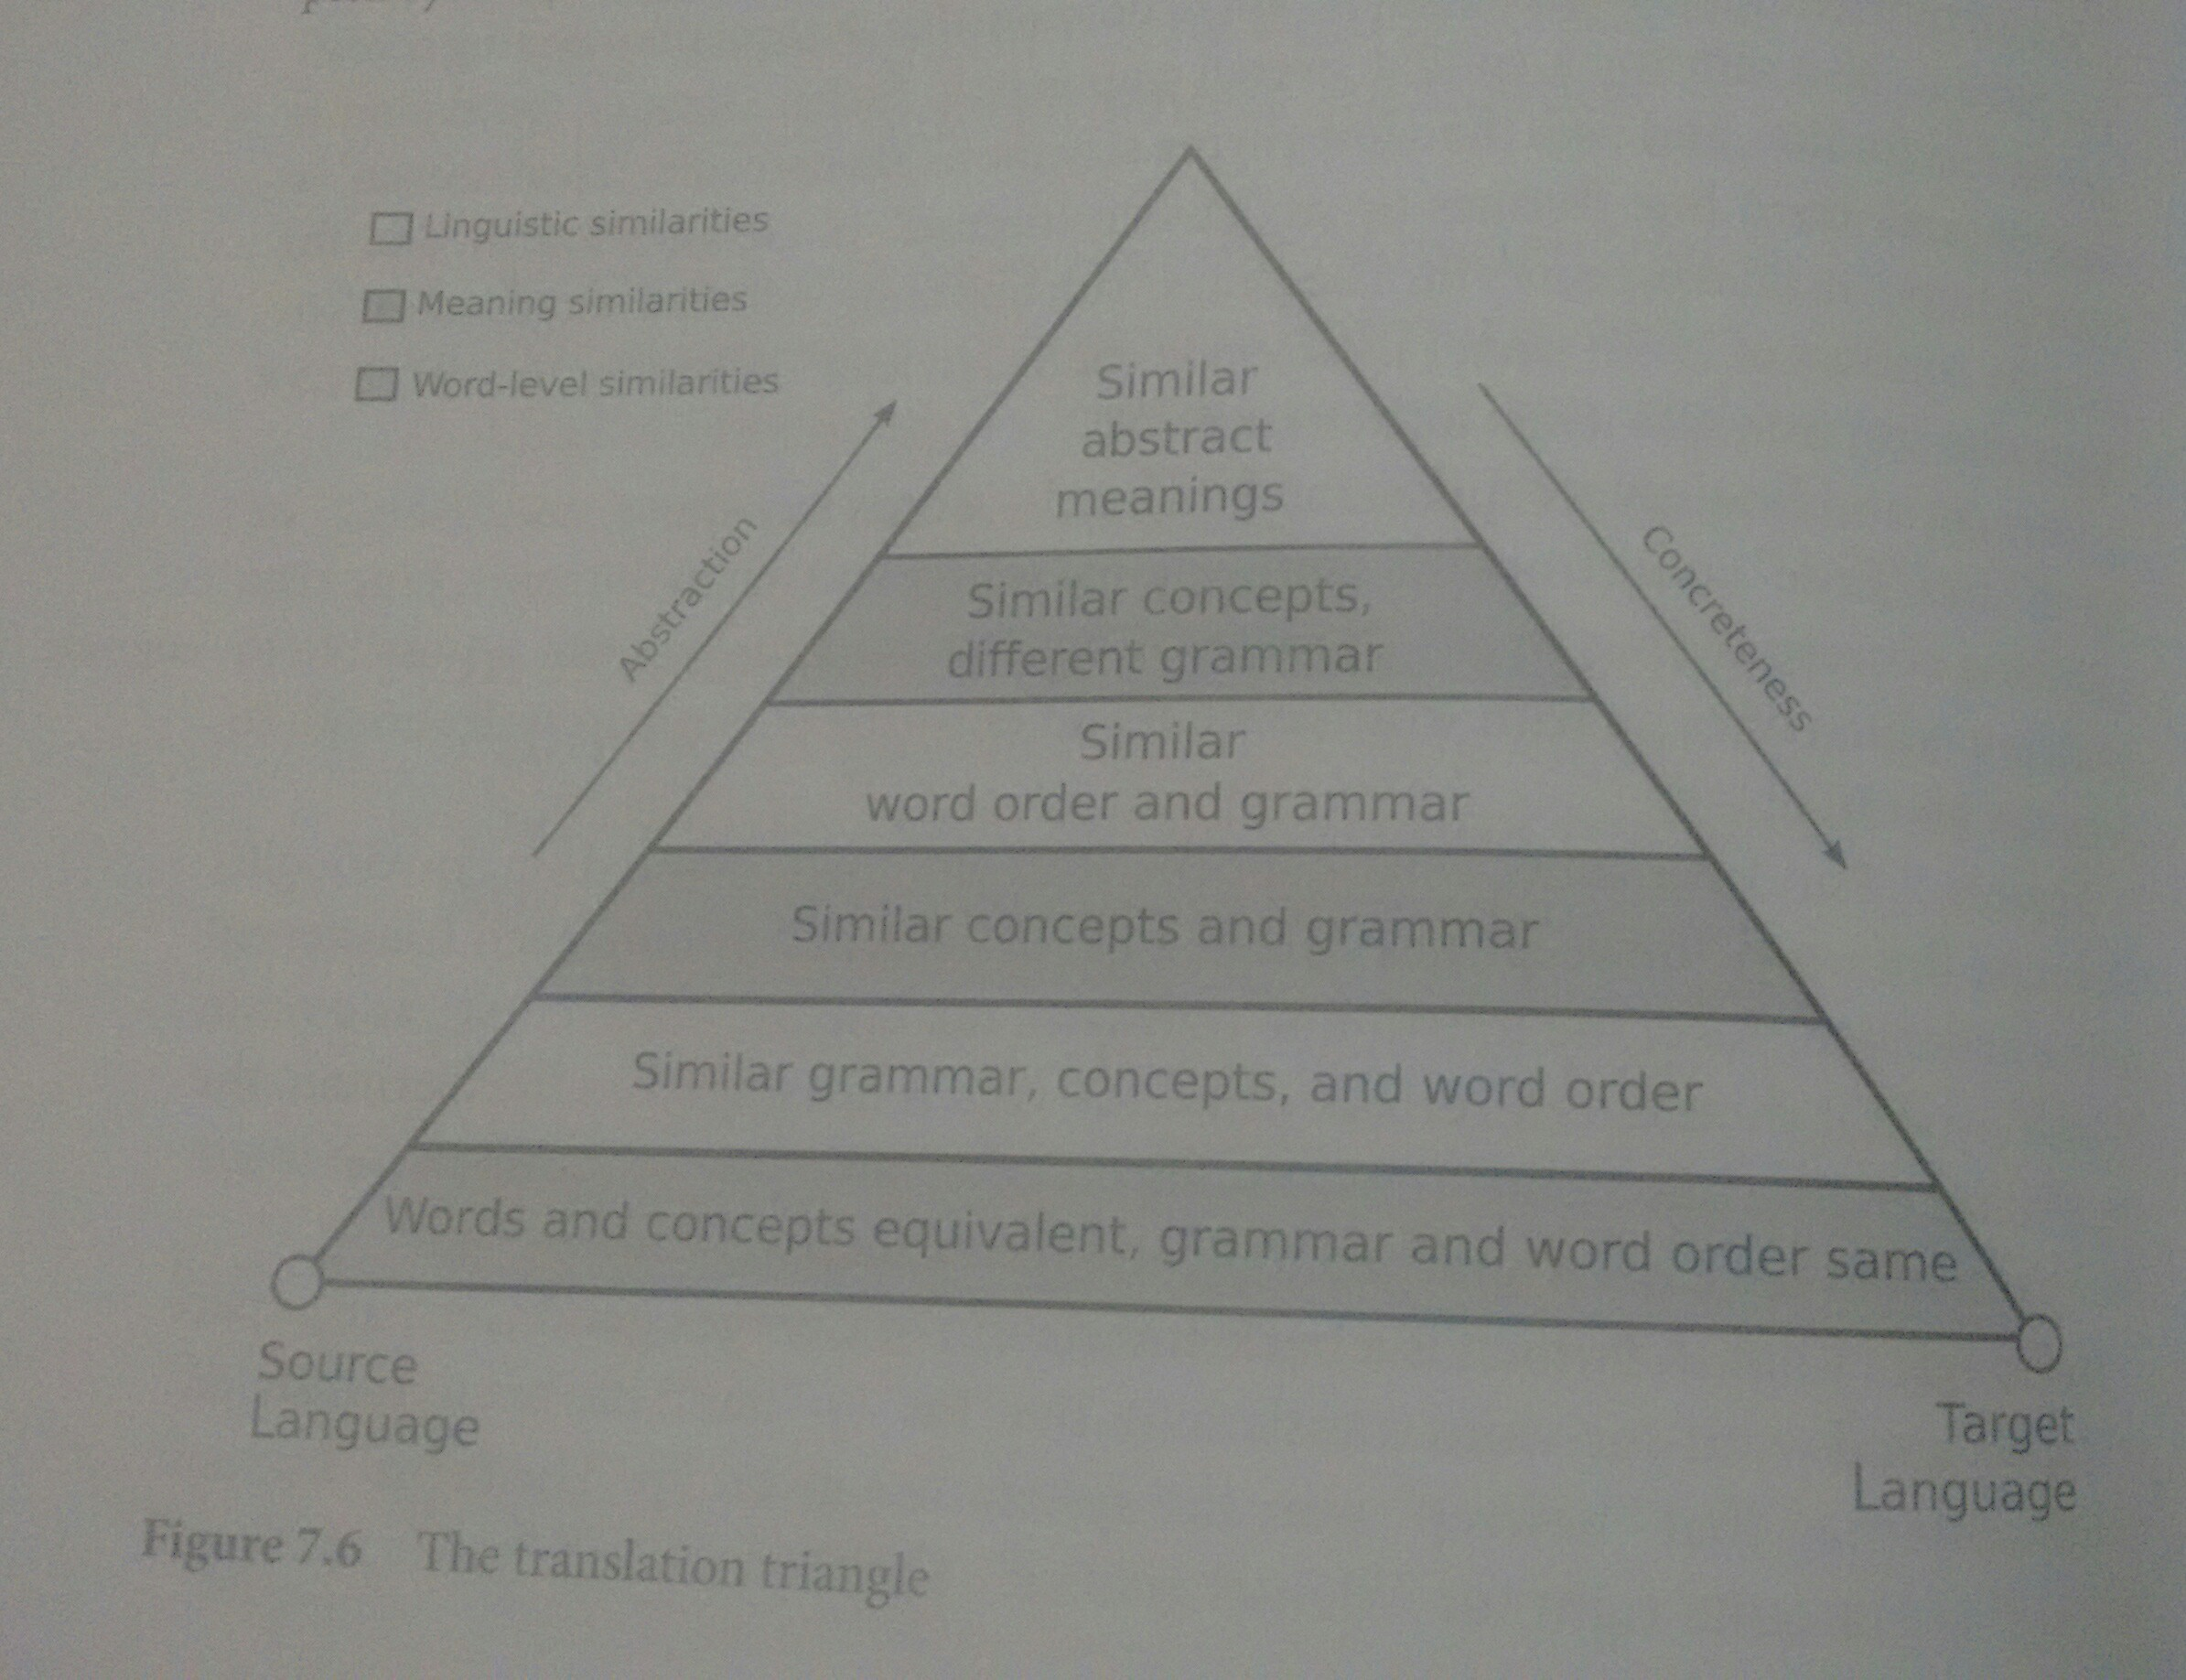
\includegraphics[width=0.7\textwidth]{MTPIC.jpg}
\pause Translation gets easier as you move higher in level of abstraction. But getting that representation is harder.
\end{frame}

\begin{frame}
\frametitle{Direct MT}
Collect dictionaries, rules about word formation (and reodering suffixes etc correctly) etc for source and target languages.
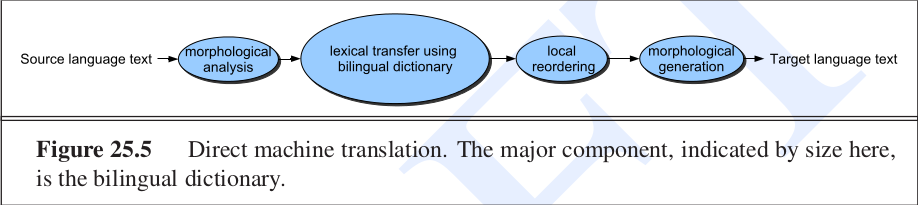
\includegraphics[width=0.9\textwidth]{directmt.png}
\end{frame}

\begin{frame}
\frametitle{Direct MT-2}
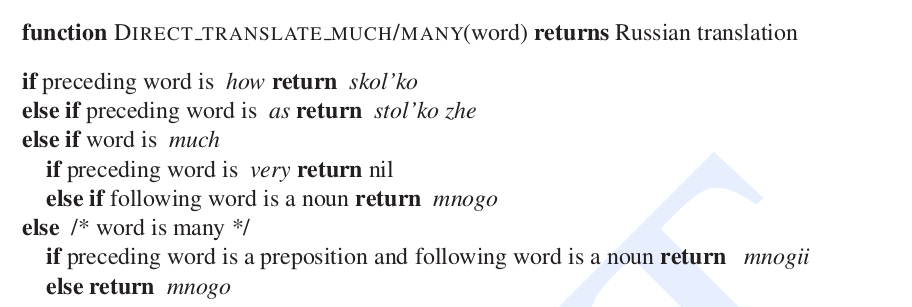
\includegraphics[width=0.9\textwidth]{directprogram.png}
\\ Main challenge with this approach? \pause - Word order, reordering is difficult.
\end{frame}

\begin{frame}
\frametitle{Syntactic Transformation based MT}
Alternative to Direct MT: Operate at the level of syntax.
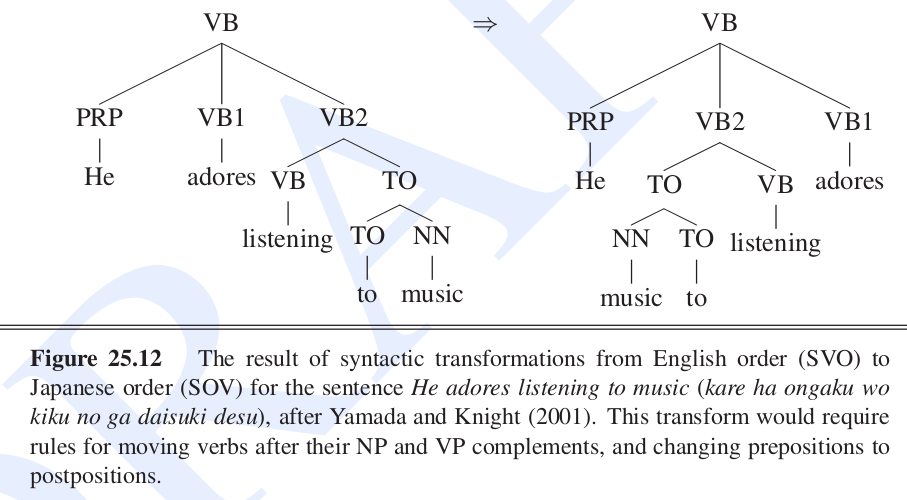
\includegraphics[width=0.9\textwidth]{transformMT.png}
\\ Main challenges: How will we know the word level translations, morphological information etc?
\end{frame}

\begin{frame}
\frametitle{Combining both ideas}
It is ofcourse a good idea to combine direct MT with syntactic rules based MT. 
\\ Main challenge with this approach ? \pause -Doing this for each and every language pair!
\end{frame}

\begin{frame}
\frametitle{Statistical MT}
\begin{itemize}
\item Modern MT is statistical and data driven i.e., it is based on:
\begin{itemize}
\item Collecting lot of parallel sentences between any two pairs
\item "learning" to align words and phrases between a source-target sentence pair
\item "learning" the probabilities of word level and phrase level translations
\item "learning" reordering and where to place a translated phrase in the process
\item  Combining all these steps to ensure translation is accurate and it is also natural in target language.
\end{itemize}
\end{itemize}
\end{frame}

\begin{frame}
\frametitle{Issues involved}
\begin{itemize}
\item How to represent sentences? How to align them in an optimal way (there are so many permutations and combinations when we don't even have a dictionary!)
\item Where do we get so much of data for any two arbitrary languages?
\item If we do sentence by sentence, how do we maintain overall text coherence?
\item If there a way to do MT via a pivot language? i.e., if I want German to Italian, but I have German to English and English to Italian, can I use those together? 
\end{itemize}
etc etc
\end{frame}

\begin{frame}
\frametitle{Noisy Channel idea for statistical MT}
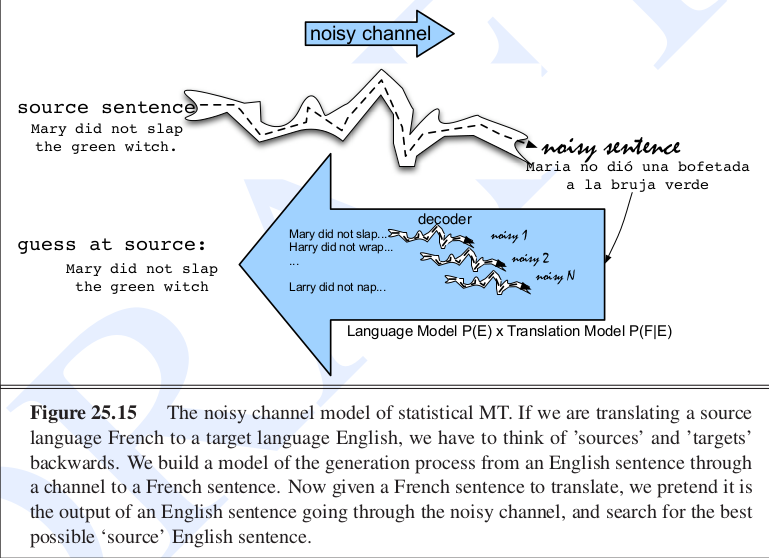
\includegraphics[width=0.9\textwidth]{noisychannel.png}
\end{frame}

\begin{frame}
\frametitle{Attendance Exercise on MT}
 There is a small news article in English and Indonesian versions.  They are not parallel versions, but are comparable.  Read the article and answer the questions in
the next page. You can work individually or in groups - up to you. This is how computers learn to create training data and learn to translate, btw. By looking at thousands and thousands of articles like this.
\end{frame}


\end{document}
